\subsection{Diseño del Amplificador de Audio}
\bigskip


\subsubsection{Primer Análisis}
 
El planteo comenzó focalizandose en un circuito mucho mas sencillo para el análisis. Por ende nos planteamos comprender el funcionamiento de un amplificador elemental con salida clase B como el de la Figura~\ref{idea_basica}.



\begin{figure}[H]
\centering
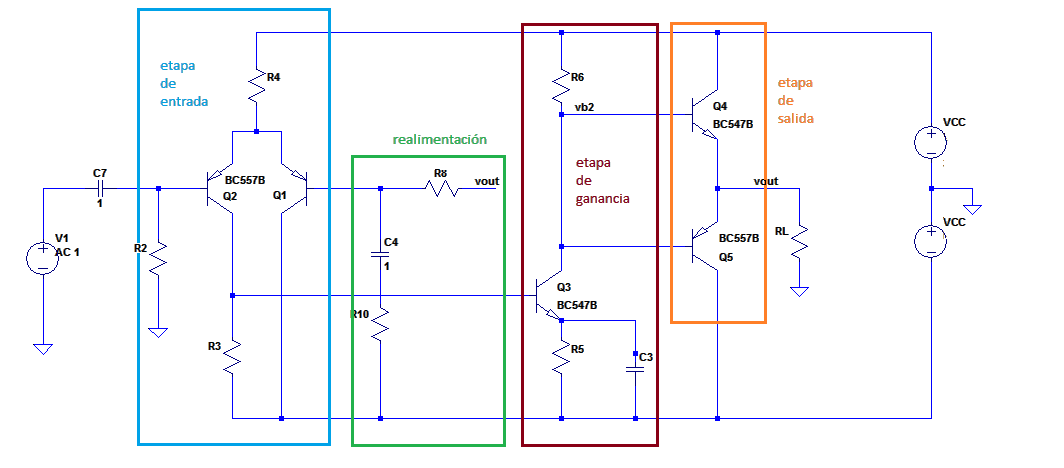
\includegraphics[width=0.8\textwidth]{img/idea_basica.png}
\caption{Amplificador simplificado.}
\label{idea_basica} 
\end{figure}

El primer desafío constó en plantear una correcta polarización. Al encontrarse el circuito realimentado negativamente es esperable que la tensión de continua en el nodo de salida $V_{out}$ sea muy cercana a cero. Este resultado puede comprenderse analizando el par diferencial y el efecto de la realimentación. Cuando el transistor Q2 se encuentre polarizado su tensión de base sea muy pequeña dado que circula una corriente baja. Por lo tanto, si la tensión $V_{out}$ no fuese un valor cercano a cero ya sea un valor negativo o positivo, produciría una tensión sobre el terminal de la base de Q1 distinto del correspondiente a Q2. Esto produciría que la corriente de Q2 se incremente o baje con respecto a la de Q1 y la salida también se vea afectada. Planteando que  $V_{out}$ aumentara:
$$
V_{out} \nearrow  ~ \Rightarrow V_{EB1} \searrow ~\Rightarrow I_{C1} \searrow ~\Rightarrow I_{C2} \nearrow ~\Rightarrow V_{B3} \nearrow ~\Rightarrow I_{C3} \nearrow \Rightarrow V_{B4} \searrow ~\Rightarrow V_{out} \searrow
$$

Siguiendo con este razonamiento si asumimos que $V_{out}$ es cercano a 0 volts. Entonces analizando el circuito llegamos a las siguientes ecuaciones:

\[
\frac{V_{CC}}{R6} = \frac{(V_{E3} - (-V_{cc})}{R5}
\]

$$
V_{E3} = V_B{3} - 0.7V
$$

Donde:
\begin{description}


\item $V_{B3} = (IC1 \times R_3 - V_{CC}) $
\item $I_{C1}=\frac{(V_{CC}-0.7V)}{2R_4}$
\item $V_{E3}= (V_{CC}-0.7) \frac{R3}{2R4} - V_{CC} - 0.7V$
\item $V_{CC} R5/R6 = \left[  (V_{CC}-0.7V) \times \frac{R_3}{2R_4} - 0.7V\right] $
\end{description}

Aproximando obtuvimos la siguiente relación:

$$ V_{CC} \times \frac{R_5}{R_6} + 0.7 =V_{CC} \times \frac{R_3}{2R_4} $$

Notando que el termino $\frac{R_5}{R_6}$ debía ser menor que la unidad debido a que $R_5$ es una resistencia de realimentación para la estabilidad de la polarización y $R_6$ es la que define la ganancia de esa etapa, y suele ser bastante alta para tener una alta ganancia de lazo abierto. 
Al tener una alta ganancia a lazo abierto la ganancia de lazo cerrado queda completamente definida por el realimentador. Observando el circuito:

$$ V_{out}= V_{in} \times \left(  1+\frac{R_8}{R_{10}} \right) ~ \Rightarrow ~ A_V= \left( 1+\frac{R_8}{R_{10}}\right) $$


Utilizando la sensibilidad requerida en las especificaciones,se estipula que al tener 1V rms en la entrada debemos tener máxima potencia de la señal de salida, asignamos a $R_8 = 22\kohm$ y a $R_{10} = 1\kohm$. De esta manera se obtiene una ganancia de 23 veces con una potencia máxima de 66 Wrms sobre una carga de $8 \ohm$ cumpliendo con los requisitos. Asignando una tensión de alimentación de $V_{cc}=35V$, simulamos el circuito:

\begin{center}
\parbox{0.5\textwidth}{
--- Operating Point ---
\begin{tabbing}
\hspace{3cm}\=\hspace{4cm}\=\hspace{5cm}\=\kill
I(Rl): \>	 -0.000492201 \>	 device$\_$current \\ 
Ie(Q1):	\> 0.000392712	\> device$\_$current \\ 
Ie(Q2):	\> 0.00116932	\> device$\_$current \\ 
I(R8):	\> -4.57521e-007\>	 device$\_$current \\ 
I(R6):	\> 0.000730688	\> device$\_$current \\ 
I(R5):	\> 0.000731219	\> device$\_$current \\ 
I(R3):	\> -0.00116632	\> device$\_$current \\ 
I(R2):	\> -1.36041e-006\>	 device$\_$current \\ 
I(R4):	\> 0.00156204	\> device$\_$current \\ 
\end{tabbing}
}
\end{center}

Los valores asignados fueron elegidos con el criterio de lograr una corriente de alrededor de 1mA para la etapa de entrada y de una relación entre $\frac{R5}{R6}$  de 0.001 veces. Obteniendo el resultado de que el circuito amplifica 22.85 veces y posee una alta inestabilidad.
Notar que el circuito simulado posee una resistencia de carga de 100 $\ohm$. Realizando una simulación habiendo compensado el circuito para que no se produzcan oscilaciones obtuvimos

\subsubsection{Etapa de Entrada}
Debido a que se piensa utilizar realimentación para mejorar las características del circuito, se implementa una entrada diferencial, cuya implementación más simple es un par diferencial. En parte porque se puede mejorar fácilmente utilizando:

\begin{itemize}
\item Fuente de corriente para su polarización, aumentando su relación de rechazo en modo común
\item Realimentaciones locales para disminuir distorsiones debido a alinealidades.
\item Un par de transistores en paralelo para mejorar la relación señal-ruido.
\item Una fuente de corriente espejo como carga para aumentar la ganancia de corriente a la salida de esta etapa y cancelar el $2^{da}$ armónica.
\end{itemize}

\bigskip
\subsubsection{Slew Rate}

El capacitor de compensación C conectado alrededor del par Darlinghton hace que esta etapa actúe como un integrador, y la corriente que carga el punto de compensación es justamente $I_x$. 
Se puede observar que la corriente máxima disponible para cargar C es 2$I_1$, donde $I_1$ es la corriente en reposo por cada dispositivo en la etapa de entrada. Es decir, a grandes valores de Vi las corrientes del par diferencial se desequilibran, $I_1$ crece hasta su valor máximo 2$I_1$ y la corriente por la otra rama del par se anula, por ende es fácil ver que por la carga activa deja de circular corriente y toda la corriente de la primer rama del par se transforma en $I_x$.
El circuito por lo tanto opera en forma no lineal. Si la etapa de entrada actuara de forma lineal produciría una corriente $I_x$ muy grande y el slew rate no produciría ninguna limitación.

\[
	V_o= \dfrac{1}{C} \int 2I_1\,\mathrm{d}t    
\]

$$
	SR=\dfrac{dVo}{dt}=\dfrac{2I_1}{C}
$$

Por lo tanto, realizando el calculo para nuestro circuito, siendo $I_1$ =2.2mA y C=120pF. Obtenemos:
$$ SR=36\dfrac{V}{\usec} $$


%El principal inconveniente al compensar el circuito por polo dominantes es que al agregar un capacitor, este modifica el ancho de banda de potencia. Esto se debe al tiempo que le toma a la etapa anterior cargar el capacitor. Debido a esto la elección del valor de este capacitor debe tener en cuenta ambos efectos y buscar una relación de compromiso entre ambos.

\bigskip
\subsubsection{Protección Contra Cortocircuitos}\label{contra_cortos} 